% ============================================================================
% Seminario: Integral de camino de Feynman en mecánica cuántica
% Asignatura: FCL1109 - Física Computacional, Universidad de El Salvador
% Autor:      José Francisco Argueta Valle
% ============================================================================
\documentclass[aspectratio=169, 11pt]{beamer}

% --- Idioma y codificación ---
\usepackage[utf8]{inputenc}
\usepackage[T1]{fontenc}
\usepackage[spanish,es-tabla]{babel}
\usepackage{csquotes}

% --- Tema y colores ---
\usetheme{Madrid}
\usecolortheme{beaver}

% --- Tipografía ---
\usepackage{lmodern}
\usepackage{microtype}

% --- Matemáticas ---
\usepackage{amsmath, amssymb}

% --- Figuras y gráficos ---
\usepackage{graphicx}
\graphicspath{{figuras/}}
\usepackage{tikz}
\usetikzlibrary{arrows.meta, positioning, shapes.geometric}

% --- Tablas ---
\usepackage{booktabs}
\usepackage{multirow}
\usepackage{tabularx}
\usepackage{array}

% --- Código fuente ---
\usepackage{listings}
\lstset{
  language=Python,
  basicstyle=\ttfamily\scriptsize,
  keywordstyle=\color{structure}\bfseries,
  commentstyle=\itshape\color{gray},
  stringstyle=\color{teal},
  showstringspaces=false,
  breaklines=true,
  columns=fullflexible,
  keepspaces=true,
  inputencoding=utf8,
  extendedchars=true,
  literate=%
    {á}{{\'a}}1 {é}{{\'e}}1 {í}{{\'i}}1 {ó}{{\'o}}1 {ú}{{\'u}}1
    {Á}{{\'A}}1 {É}{{\'E}}1 {Í}{{\'I}}1 {Ó}{{\'O}}1 {Ú}{{\'U}}1
    {ñ}{{\~n}}1 {Ñ}{{\~N}}1 {ü}{{\"u}}1 {ö}{{\"o}}1,
}

% --- Bibliografía ---
\usepackage[backend=biber, style=numeric, sorting=none]{biblatex}
\addbibresource{referencias.bib}

% --- Configuración adicional ---
\setbeamertemplate{navigation symbols}{}
\setbeamertemplate{bibliography item}{\insertbiblabel}

% ============================================================================
% Metadatos
% ============================================================================
\title[Integral de camino de Feynman]{Integral de camino de Feynman en mecánica cuántica}
\subtitle{Monte Carlo cuántico con el algoritmo de Metropolis}
\author[J. F. Argueta]{José Francisco Argueta Valle}
\institute[UES - FCL1109]{Escuela de Física, Facultad de Ciencias Naturales y Matemática\\
Universidad de El Salvador\\[4pt]
Seminario de Física Computacional (FCL1109)}
\date{19 de junio de 2026}

% ============================================================================
\begin{document}

% --- Portada ---
\begin{frame}
  \titlepage
\end{frame}

% --- Índice ---
\begin{frame}{Contenido}
  \tableofcontents
\end{frame}

% ============================================================================
\section{Introducción}
% ============================================================================

\begin{frame}{Motivación: otra forma de ver la mecánica cuántica}
  \small
  Feynman buscaba una formulación de la mecánica cuántica distinta de la imagen
  de Schrödinger, con una conexión más directa con la mecánica clásica. Dirac
  había sugerido el principio de mínima acción como el límite $\hbar \to 0$ de un
  principio cuántico de acción~\parencite{sakurai_1967, feynman_1948}.

  \vspace{0.25cm}
  \begin{block}{Las dos imágenes}
    \begin{itemize}\setlength\itemsep{3pt}
      \item \textbf{Schrödinger:} una ecuación diferencial para la función de onda
            $\psi(x,t)$ que se propaga en el tiempo.
      \item \textbf{Feynman:} la amplitud de ir de un punto a otro es una
            suma sobre todos los caminos del espacio-tiempo.
    \end{itemize}
  \end{block}
\end{frame}

\begin{frame}{La idea central: suma sobre caminos}
  \small
  Contribuyen todos los caminos, cada uno con un peso $e^{iS/\hbar}$ que depende de
  su acción. El camino clásico es el de acción mínima y el más probable.

  \vspace{0.1cm}
  \begin{columns}
    \begin{column}{0.50\textwidth}
      \centering
      \begin{tikzpicture}[scale=0.85]
        \draw[->] (0,0) -- (4.6,0) node[right] {\scriptsize $x$};
        \draw[->] (0,0) -- (0,3.6) node[above] {\scriptsize $t$};
        \fill (0.8,0.3) circle (2pt) node[below] {\scriptsize $A$};
        \fill (3.6,3.2) circle (2pt) node[above] {\scriptsize $B$};
        \draw[very thick, structure] (0.8,0.3) .. controls (1.6,1.4) and (2.8,2.2) .. (3.6,3.2);
        \draw[dashed, gray] (0.8,0.3) .. controls (0.4,1.9) and (3.0,1.6) .. (3.6,3.2);
        \draw[dashed, gray] (0.8,0.3) .. controls (2.6,0.9) and (1.2,2.8) .. (3.6,3.2);
        \draw[dashed, gray] (0.8,0.3) .. controls (2.2,2.0) and (4.2,2.5) .. (3.6,3.2);
      \end{tikzpicture}
    \end{column}
    \begin{column}{0.50\textwidth}
      \begin{itemize}\setlength\itemsep{4pt}
        \item Línea gruesa: trayectoria clásica $\bar{x}(t)$.
        \item Líneas discontinuas: otros caminos que muestrea la partícula.
        \item El peso $e^{iS/\hbar}$ asigna una fase a cada camino.
      \end{itemize}
    \end{column}
  \end{columns}
\end{frame}

% ============================================================================
\section{Teoría}
% ============================================================================

\begin{frame}{Propagador, acción e integral de camino}
  \small
  La función de onda se propaga mediante el propagador (función de Green)
  $G$~\parencite{feynman_hibbs_1965}:
  \begin{equation*}
    \psi(x_b, t_b) = \int dx_a\; G(x_b, t_b; x_a, t_a)\, \psi(x_a, t_a).
  \end{equation*}
  Feynman postuló que $G$ es la suma sobre todos los caminos, cada uno ponderado
  por su acción $S = \int L\, dt$, con $L = T - V$~\parencite{feynman_1948}:
  \begin{equation*}
    G(b, a) = \sum_{\text{caminos}} e^{\, i S[b,a]/\hbar}
      \qquad \text{(integral de camino)}.
  \end{equation*}
\end{frame}

\begin{frame}{Límite clásico y tiempo imaginario}
  \small
  Como $\hbar \approx 10^{-34}$~J\,s, la acción es enorme ($S/\hbar \gtrsim 10^{20}$):
  las fases de caminos vecinos se cancelan salvo cerca del camino de acción mínima.
  Así emerge la trayectoria clásica.

  \vspace{0.2cm}
  El truco de cálculo es rotar a \textbf{tiempo imaginario} $t \to -i\tau$. La
  exponencial deja de oscilar y se vuelve un peso real $e^{-S_E}$. Para tiempos
  imaginarios grandes domina el estado de menor energía~\parencite{landau_paez_2018}:
  \begin{equation*}
    |\psi_0(x)|^2 = \lim_{\tau \to \infty} e^{E_0 \tau}\, G(x, -i\tau; x, 0).
  \end{equation*}
\end{frame}

\begin{frame}{Discretización en una red de espacio-tiempo}
  \small
  Se coloca el camino en una red: posiciones $x_i$ en cortes de tiempo imaginario
  separados $\varepsilon$. La acción euclidiana del oscilador armónico
  ($\hbar = m = \omega = 1$) es una suma sobre eslabones:
  \begin{equation*}
    S_E = \sum_{i} \left[\, \frac{(x_{i+1} - x_i)^2}{2\varepsilon}
      + \frac{\varepsilon\, \omega^2}{2}\, x_i^2 \,\right]
      = \sum_i (\text{cinética} + \text{potencial}).
  \end{equation*}

  \begin{block}{Resultado exacto de comparación}
    $\displaystyle |\psi_0(x)|^2 = \frac{1}{\sqrt{\pi}}\, e^{-x^2}$,
    \quad $E_0 = \tfrac{1}{2}\hbar\omega$, \quad $\langle x^2 \rangle = \tfrac{1}{2}$.
  \end{block}
\end{frame}

% ============================================================================
\section{Algoritmo y código}
% ============================================================================

\begin{frame}{Qué queremos calcular y cómo}
  \small
  \textbf{Objetivo:} obtener la densidad del estado fundamental $|\psi_0(x)|^2$ y la
  energía $E_0$ del oscilador, sin resolver la ecuación de Schrödinger, evaluando la
  integral de muchas dimensiones del peso $e^{-S_E}$ por Monte Carlo.

  \vspace{0.25cm}
  \textbf{Estrategia} (tres pasos):
  \begin{enumerate}\setlength\itemsep{3pt}
    \item Representar el camino como un arreglo de $N$ posiciones $x_i$ en una red.
    \item Muestrear caminos con probabilidad $\propto e^{-S_E}$ usando Metropolis.
    \item Acumular las posiciones visitadas en un histograma: ese histograma
          \emph{es} $|\psi_0(x)|^2$, y de $\langle x^2\rangle$ se obtiene $E_0$.
  \end{enumerate}
\end{frame}

\begin{frame}{Algoritmo de Metropolis}
  \small
  El peso $e^{-S_E}$ se muestrea con el algoritmo de Metropolis, el mismo de la
  física estadística~\parencite{metropolis_1953, creutz_freedman_1981}:

  \vspace{0.15cm}
  \begin{enumerate}\setlength\itemsep{2pt}
    \item Inicializar el camino (todos los eslabones en $x = 0$).
    \item Repetir muchas veces:
      \begin{itemize}\setlength\itemsep{1pt}
        \item Elegir un eslabón $i$ y proponer $x_i \to x_i + \delta$.
        \item Calcular el cambio de acción $\Delta S$.
        \item Aceptar si $\Delta S \leq 0$, o si $e^{-\Delta S/\hbar} >$ aleatorio.
        \item Si no, rechazar y restaurar $x_i$.
        \item Acumular la posición en el histograma de $|\psi_0|^2$.
      \end{itemize}
  \end{enumerate}
\end{frame}

\begin{frame}{Estructura del programa}
  \small
  El script \texttt{qmc\_camino\_feynman.py} se organiza en pocas funciones:

  \vspace{0.2cm}
  \begin{itemize}\setlength\itemsep{4pt}
    \item \texttt{energia\_total(camino)}: acción euclidiana completa (diagnóstico).
    \item \texttt{barrido\_metropolis(...)}: actualiza una vez cada eslabón del camino.
    \item \texttt{simular(...)}: termaliza, mide y acumula el histograma y $\langle x^2\rangle$.
    \item \texttt{densidad\_analitica(x)}: la curva exacta de comparación.
    \item \texttt{main()}: ejecuta la simulación y genera las cuatro figuras.
  \end{itemize}

  \vspace{0.2cm}
  Parámetros principales: \texttt{N\_eslabones=200}, \texttt{eps=0.25},
  \texttt{omega=1.0}, \texttt{barridos\_medicion=40000}.
\end{frame}

\begin{frame}[fragile]{La acción discretizada en código}
  \small
  La función calcula la energía cinética (diferencias entre eslabones contiguos) y
  la potencial del oscilador, con frontera periódica vía \texttt{np.roll}:
  \vspace{0.15cm}
\begin{lstlisting}
def energia_total(camino, eps, omega, masa):
    # x_{i+1} - x_i con frontera periódica
    dx = np.roll(camino, -1) - camino
    cinetica = 0.5 * masa * np.sum(dx**2) / eps
    potencial = 0.5 * masa * omega**2 * eps * np.sum(camino**2)
    return cinetica + potencial
\end{lstlisting}
  \vspace{0.1cm}
  En el muestreo no se recalcula toda la acción: solo cambia el aporte local del
  eslabón que se mueve, lo que hace cada paso muy barato.
\end{frame}

\begin{frame}[fragile]{Un barrido de Metropolis}
  \small
  Esquema rojo-negro: los eslabones que no son vecinos se actualizan a la vez, lo
  que vectoriza el barrido con \texttt{numpy}.
  \vspace{0.1cm}
\begin{lstlisting}
# Propuesta de desplazamiento para los eslabones de un color
x_nuevo = x_viejo + paso * (2*rng.random(idx.size) - 1)

# Acción local antes y después (solo términos que dependen de x_i)
s_viejo = ((x_viejo-vec_izq)**2 + (vec_der-x_viejo)**2)/(2*eps) \
          + 0.5*omega**2*eps*x_viejo**2
s_nuevo = ((x_nuevo-vec_izq)**2 + (vec_der-x_nuevo)**2)/(2*eps) \
          + 0.5*omega**2*eps*x_nuevo**2
delta_s = s_nuevo - s_viejo

# Criterio de Metropolis (aceptar o rechazar, vectorizado)
acepta = (delta_s <= 0) | (rng.random(idx.size) < np.exp(-delta_s/hbar))
camino[idx] = np.where(acepta, x_nuevo, x_viejo)
\end{lstlisting}
\end{frame}

\begin{frame}[fragile]{Medición: acumular el histograma}
  \small
  Tras termalizar, cada barrido aporta sus $N$ posiciones al histograma y a la suma
  de $x^2$. El histograma normalizado es la densidad $|\psi_0(x)|^2$:
  \vspace{0.15cm}
\begin{lstlisting}
for k in range(barridos_medicion):
    barrido_metropolis(camino, eps, omega, masa, paso, hbar, rng)
    conteo, _ = np.histogram(camino, bins=bordes_hist)
    histograma += conteo            # acumula |psi_0(x)|^2
    suma_x2 += np.sum(camino**2)    # para <x^2> y la energía

# normalizar para que el histograma integre a 1
densidad = histograma / (np.sum(histograma) * ancho)
\end{lstlisting}
  \vspace{0.1cm}
  La energía sale del virial: $E_0 = \omega^2 \langle x^2 \rangle$.
\end{frame}

% ============================================================================
\section{Resultados}
% ============================================================================

\begin{frame}{Caminos muestreados y trayectoria clásica}
  \centering
  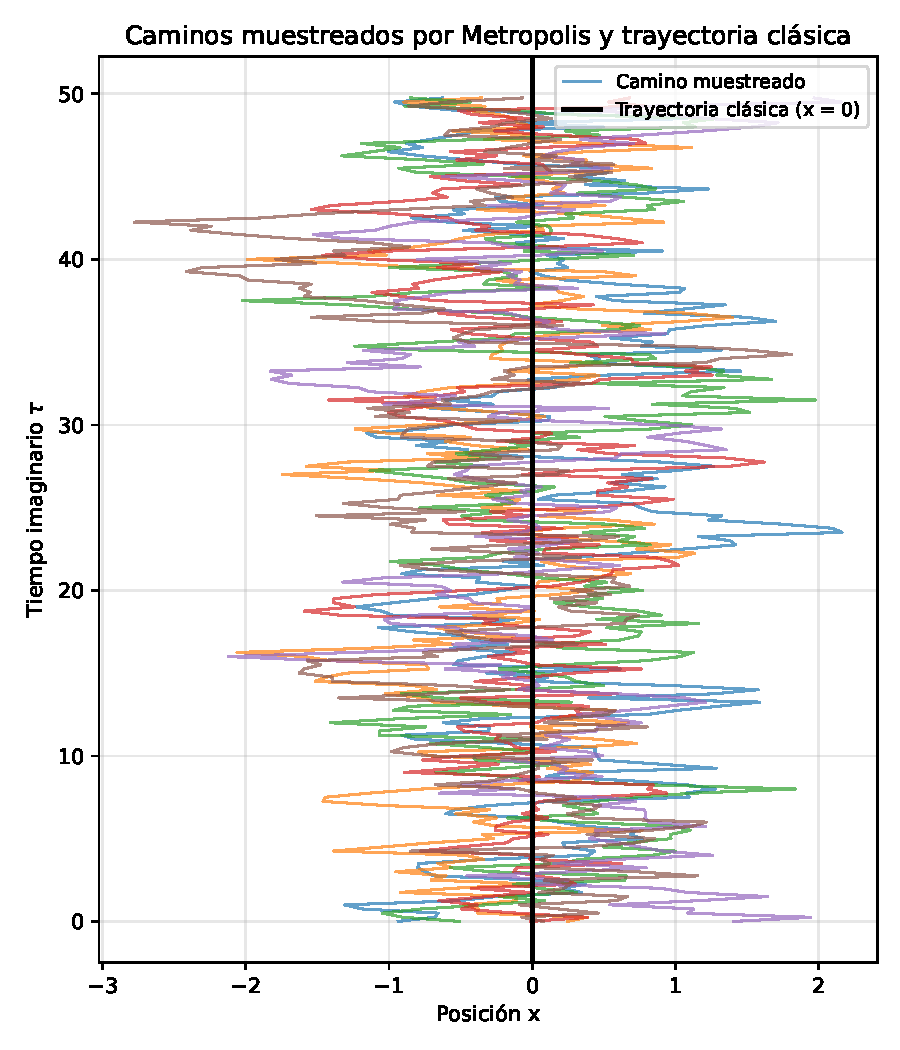
\includegraphics[height=0.78\textheight]{caminos_espaciotemporales.pdf}
\end{frame}

\begin{frame}{Función de onda del estado fundamental}
  \centering
  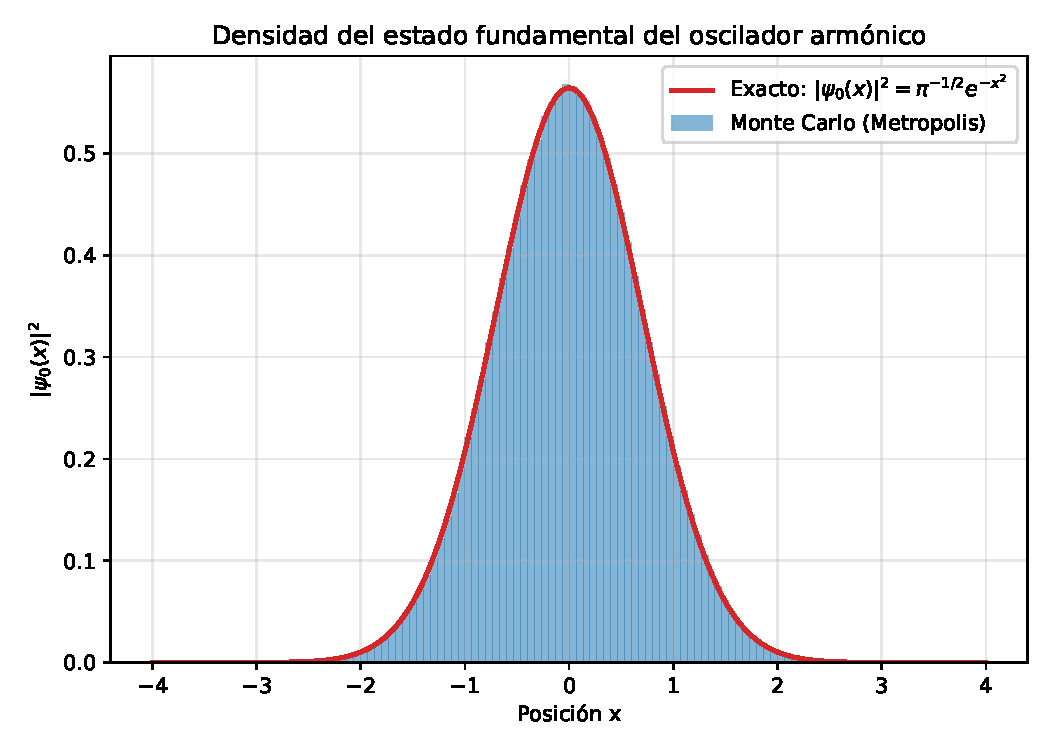
\includegraphics[height=0.70\textheight]{funcion_onda_fundamental.pdf}

  {\scriptsize El histograma de Monte Carlo reproduce la gaussiana exacta $\pi^{-1/2} e^{-x^2}$.}
\end{frame}

\begin{frame}{Convergencia de la energía}
  \centering
  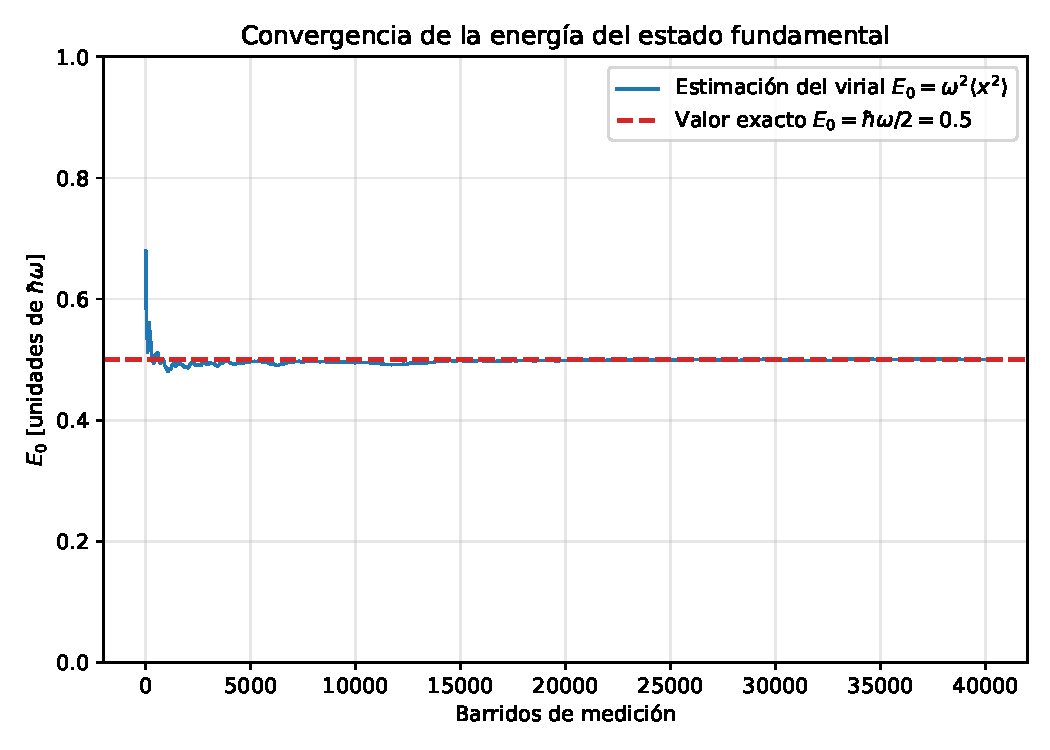
\includegraphics[height=0.70\textheight]{convergencia_energia.pdf}

  {\scriptsize $E_0 = \omega^2\langle x^2\rangle$ converge a $\hbar\omega/2 = 0.5$ (se obtuvo $0.5001$).}
\end{frame}

\begin{frame}{Efecto de $\hbar$ sobre las fluctuaciones}
  \small
  \begin{columns}
    \begin{column}{0.60\textwidth}
      \centering
      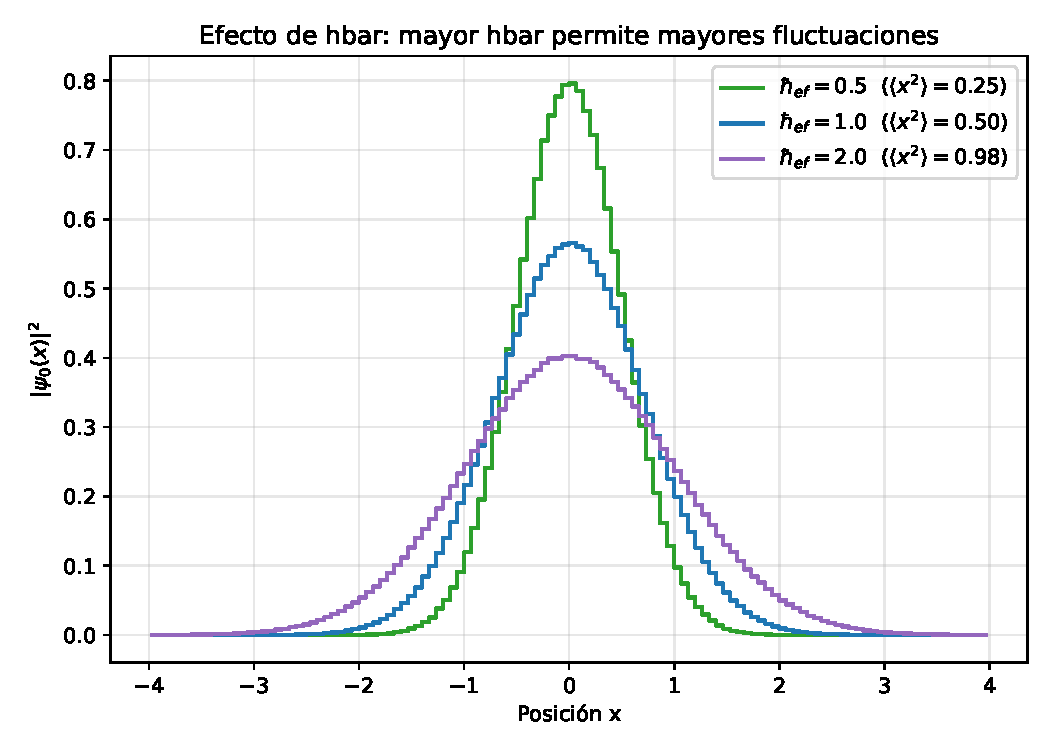
\includegraphics[width=\textwidth]{efecto_hbar.pdf}
    \end{column}
    \begin{column}{0.40\textwidth}
      Al aumentar $\hbar$ se permiten mayores fluctuaciones:
      \begin{itemize}\setlength\itemsep{3pt}
        \item la distribución se ensancha,
        \item $\langle x^2 \rangle$ crece como $\hbar/2$,
        \item en el límite $\hbar \to 0$ solo sobrevive el camino clásico.
      \end{itemize}
    \end{column}
  \end{columns}
\end{frame}

% ============================================================================
\section{Relación con la asignatura}
% ============================================================================

\begin{frame}{Conexiones con los temas del curso}
  \small
  \begin{itemize}\setlength\itemsep{6pt}
    \item \textbf{Metropolis y Monte Carlo} (termodinámica y física estadística,
          Cap.~7 de Landau): el mismo algoritmo que muestrea el modelo de Ising.
    \item \textbf{Ecuación de difusión} (Cap.~4): Schrödinger en tiempo imaginario
          es una ecuación de difusión, y por eso $e^{iS/\hbar}$ pasa a ser $e^{-S_E}$.
    \item \textbf{Oscilador armónico} (Cap.~3 clásico, Cap.~6 cuántico): el sistema
          de prueba ya estudiado en clase.
    \item \textbf{Números aleatorios y muestreo}, base de los métodos Monte Carlo.
    \item \textbf{Trayectoria clásica} como solución de las ecuaciones de movimiento
          (EDOs con rk4): es el límite $\hbar \to 0$ de la suma.
  \end{itemize}
\end{frame}

% ============================================================================
\section{Conclusiones}
% ============================================================================

\begin{frame}{Conclusiones}
  \small
  \begin{itemize}\setlength\itemsep{6pt}
    \item La integral de camino reformula la mecánica cuántica como suma sobre
          caminos y reproduce la misma física que la imagen de Schrödinger.
    \item En tiempo imaginario, el Monte Carlo con Metropolis recupera
          $|\psi_0(x)|^2 = \pi^{-1/2} e^{-x^2}$ y $E_0 = 0.5\,\hbar\omega$ (se obtuvo $0.5001$).
    \item El camino clásico domina; las fluctuaciones crecen con $\hbar$, lo que
          ilustra de forma directa el límite clásico.
    \item El método enlaza la mecánica cuántica con los métodos Monte Carlo y de
          ecuaciones en derivadas parciales vistos en la asignatura.
  \end{itemize}
\end{frame}

% ============================================================================
\section*{Referencias}
% ============================================================================

\begin{frame}[allowframebreaks]{Referencias}
  \scriptsize
  \printbibliography[heading=none]
\end{frame}

% --- Slide de cierre ---
\begin{frame}[plain]
  \centering
  \vfill
  {\Large \textbf{Gracias por su atención}}

  \vspace{1cm}
  {\normalsize Preguntas y comentarios}
  \vfill
\end{frame}

% ============================================================================
\appendix
% ============================================================================

\begin{frame}[allowframebreaks, fragile]{Apéndice: código completo}
  \scriptsize
  Archivo \texttt{codigo/qmc\_camino\_feynman.py} (adaptación del listado 6.24,
  \texttt{QMC.py}, de Landau y Páez).
  \vspace{0.2cm}
  \lstinputlisting[basicstyle=\ttfamily\tiny]{codigo/qmc_camino_feynman.py}
\end{frame}

\end{document}
